\begin{figure}[htbp]
\centering
\shorthandoff{<>}
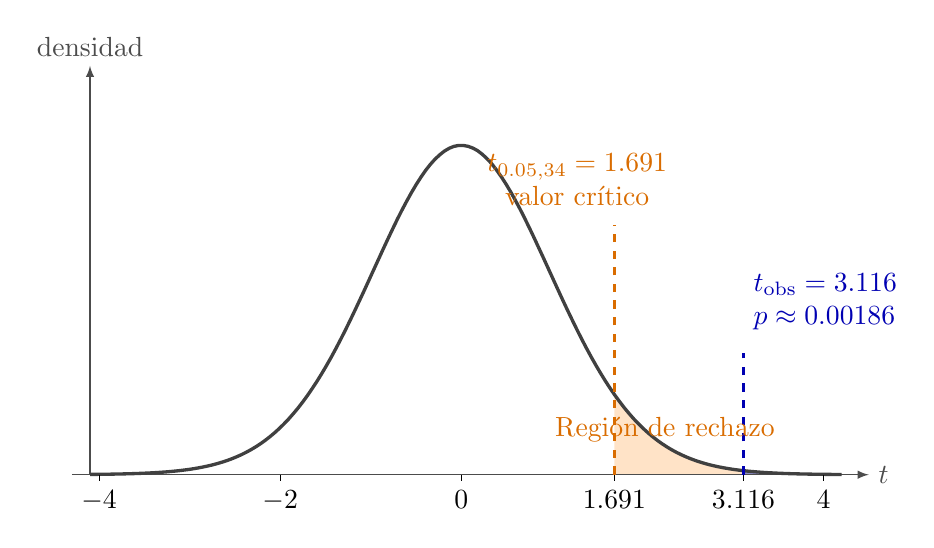
\begin{tikzpicture}[x=1.15cm,y=4.4cm,font=\normalsize,>=latex]
  \fill[orange!22]
    (1.691,0)
    -- plot[domain=1.691:4.2,samples=100]
      (\x,{0.9504*(1+\x*\x/34)^(-17.5)})
    -- (4.2,0) -- cycle;
  \fill[blue!50!black!45]
    (3.116,0)
    -- plot[domain=3.116:4.2,samples=70]
      (\x,{0.9504*(1+\x*\x/34)^(-17.5)})
    -- (4.2,0) -- cycle;
  \draw[->,black!70] (-4.3,0) -- (4.5,0) node[right] {$t$};
  \draw[->,black!70] (-4.1,0) -- (-4.1,1.18) node[above] {densidad};
  \draw[black!75,very thick,domain=-4.1:4.2,samples=160]
    plot (\x,{0.9504*(1+\x*\x/34)^(-17.5)});
  \draw[dashed,orange!85!black,thick] (1.691,0) -- (1.691,0.72);
  \draw[dashed,blue!70!black,thick] (3.116,0) -- (3.116,0.35);
  \node[above,align=center,orange!85!black] at (1.28,0.75)
    {$t_{0.05,34}=1.691$\\valor crítico};
  \node[above right,align=left,blue!70!black] at (3.12,0.39)
    {$t_{\mathrm{obs}}=3.116$\\$p\approx0.00186$};
  \node[orange!85!black] at (2.25,0.13) {Región de rechazo};
  \foreach \x/\etiqueta in {-4/-4,-2/-2,0/0,1.691/1.691,3.116/3.116,4/4}{
    \draw (\x,0) -- (\x,-0.018) node[below] {$\etiqueta$};
  }
\end{tikzpicture}
\shorthandon{<>}
\caption{Distribución $t$ aproximada con $\nu=34$ grados de libertad para la prueba unilateral. La región naranja comienza en el valor crítico; el área azul, contenida en ella y a la derecha del estadístico observado, representa el valor-$p$. Como $t_{\mathrm{obs}}>t_{0.05,34}$, se rechaza $H_0$.}
\label{fig:prueba-t}
\end{figure}